\documentclass{article}
\usepackage{listings, xcolor, graphicx}
\setlength{\parindent}{0pt}

\definecolor{lgray}{rgb}{0.95, 0.95, 0.95}
\definecolor{lgray2}{rgb}{0.75, 0.75, 0.75}

\lstset{
  aboveskip=10pt,
  belowskip=10pt,
  frame=leftline,
  xleftmargin=15pt,
  framexleftmargin=20pt,
  breaklines=true,
  basicstyle=\small,
  showstringspaces=false,
  backgroundcolor=\color{lgray},
  rulecolor=\color{lgray2}
}

\title{CS135; Control Structures II (Repetition)}
\author{Gael Zarco}
\date{\today}

\begin{document}

\maketitle

C++ has three repetition, or looping, structures that allow you to repeat a set of statement until certain conditions are men.

\section{\texttt{while} Looping (Repetition) Structure}

\begin{lstlisting}[language=C++, caption={\texttt{while} Loop Syntax}]
while (expression)
	statement;
\end{lstlisting}
\textit{Statement can be simple or compound statement.}

\vspace{8pt}
Execution Flow:
\begin{center}
    
\includegraphics[width=0.9\textwidth]{while-exec-flow.png}
\end{center}

\vspace{8pt}
\texttt{expression} acts as a \textbf{Decision Maker} and is usually a logical expression.
\begin{itemize}
    \item Provides an entry condition to the loop.
    \item If initially \texttt{true}, loop starts.
    \item Re-evaluates on each iteration, continues if \texttt{true}.
    \item Exits loop when \texttt{false}.
\end{itemize}

\textbf{Infinite Loops} are loops that execute endlessly (no exit case).

\vspace{8pt}
\texttt{statement} is the body of the loop.

\begin{lstlisting}[language=C++, caption={\texttt{while} Loop Example Program}, numbers=left]
#include <iostream>

using namespace std;

int main() {
  int calBurnedInADay;
  int calBurnedInAWeek;
  int day;

  day = 1;
  calBurnedInAWeek = 0;

  while (day <= 7) {
    cout << "Enter calories burned day " << day << ": ";
    cin >> calBurnedInADay;
    cout << endl;
    calBurnedInAWeek = calBurnedInAWeek + calBurnedInADay;
    day = day + 1;
  }
   
  cout << "Average number of calories burned each day: "
  << calBurnedInAWeek / 7 << endl;

  return 0;
}
\end{lstlisting}

\texttt{day} in the example program above is known as the \textbf{Loop Control
Variable (LCV)}.

\vspace{8pt}
Loop Control Variables:

\begin{enumerate}
    \item Must be initialized before the \texttt{while} loop.
    \item Must result in a \texttt{false} expression evaluation at a certain point.
\end{enumerate}

Be careful of where in the loop, LCVs are manipulated. This can change the behavior of the loop.

\subsection{Case 1: Counter-Controlled \texttt{while} Loops}
\textbf{Counter-Controlled \texttt{while} Loop} is a loop in
which the LCV serves as a \textit{counter} that dictates how many times the loop iterates or executes.
\begin{itemize}
  \item That is, \texttt{statement} is executed \textit{n} times.
\end{itemize}

\begin{lstlisting}[language=C++, caption={Counter-Controlled \texttt{while} Loop
  Example}, numbers=left]
counter = 0;

while (counter < N) {
  // Code that does something...
  counter++
}
\end{lstlisting}

\subsection{Case 2: Sentinel-Controlled \texttt{while} Loops}

Last entry in a set of data is known as the \textbf{sentinel} and this value
tells the loop to stop.

\begin{itemize}
  \item if \texttt{item != sentinel} $\rightarrow$ \texttt{statement}.
\end{itemize}

The \texttt{while} loop continues to execute as long as the program has not read
the \texttt{sentinel}.

\vspace{8pt}
Such a loop is known as a \textbf{Sentinel-Controlled \texttt{while} Loop}.

\begin{lstlisting}[language=C++, caption={Sentinel-Controlled \texttt{while} Loop
  Syntax}, numbers=left]
cin >> variable;

while (variable != sentinel) {
  // Code that does something...
  cin >> variable;
}
\end{lstlisting}

\subsection{Case 3: Flag-Controlled \texttt{while} Loops}

\textbf{Flag-Controlled \texttt{while} Loops} use a \texttt{bool} variable to
control the loop.

\vspace{8pt}
A \textbf{Flag Variable} is a \texttt{bool} variable that indicates whether a
condition is \texttt{true} or \texttt{false}.
\begin{itemize}
  \item Generally named for the \texttt{true} state of the condition. \textit{i.e. isFound, isTallEnough, etc}.
\end{itemize}

\begin{lstlisting}[language=C++, caption={Flag-Controlled \texttt{while} Loop
  Example}, numbers=left]
isFound = false;

while (!isFound) {
  // Code that does something...
  if (expression)
    isFound = true;
  }
}
\end{lstlisting}

\subsection{Case 4: EOF-Controlled \texttt{while} Loops}

Until now, input stream variables such as \texttt{cin} and the extraction
operator, \texttt{>>}, have been used to read and store data in variables.
However, The input stream variable can also return a value after reading data,
as follows:
\begin{enumerate}
  \item If the program has reached the end of the input data, the input stream
    var returns \texttt{false}.
  \item If the program reads any faulty data, the input stream enters the fail
    state. Because of this, any attempt to use that stream is ignored. In this
    case, the input stream var returns \texttt{false}.
  \item In any other case besides (1) and (2), the input stream var returns
    \texttt{true}.
\end{enumerate}

\textbf{EOF-Controlled \texttt{while} Loops} are best used at times where
selecting a good sentinel value is difficult or for programs where the data-file
is altered.
\begin{itemize}
  \item Someone could potentially erase the sentinel value or add past the
    value.
\end{itemize}

\begin{lstlisting}[language=C++, caption={EOF-Controlled \texttt{while} Loop
  Example}, numbers=left]
cin >> variable;

while (cin) {
  // Code that does something...
  cin >> variable;
}
\end{lstlisting}


\subsection{\texttt{eof} Function}

The \texttt{eof} function allows you to check if you have reached the
end-of-file status on an input stream variable.
\begin{itemize}
  \item Member of the data type \texttt{istream}.
  \item Logical expression; returns a boolean value.
\end{itemize}

\begin{lstlisting}[language=C++, caption={\texttt{eof} Function Syntax}]
istreamVar.eof()
\end{lstlisting}
\textit{istreamVar is an input variable stream, such as cin}.

\begin{lstlisting}[language=C++, caption={\texttt{eof} Example},
  numbers=left]
ifstream infile;
char ch;

infile.open("inputDat.dat");

infile.get(ch);

while(!infile.eof()) {
  cout << ch;
  infile.get(ch);
}
\end{lstlisting}

\section{\texttt{for} Looping (Repetition) Structure}

A counter-focused looping structure.

\begin{lstlisting}[language=C++, caption={\texttt{for} Loop Syntax}]
for(initial statement; loop condition; update statement)
  statement;
\end{lstlisting}
\textit{Statement can be a simple or compound statement.}

\vspace{8pt}
The \texttt{initial statement}, \texttt{loop condition}, and \texttt{update
statement} control the \texttt{statement} of the \texttt{for} loop.
\begin{itemize}
  \item These are known as the \texttt{for} loop control statements.
\end{itemize}

\vspace{8pt}
Execution Flow:
\begin{center}
    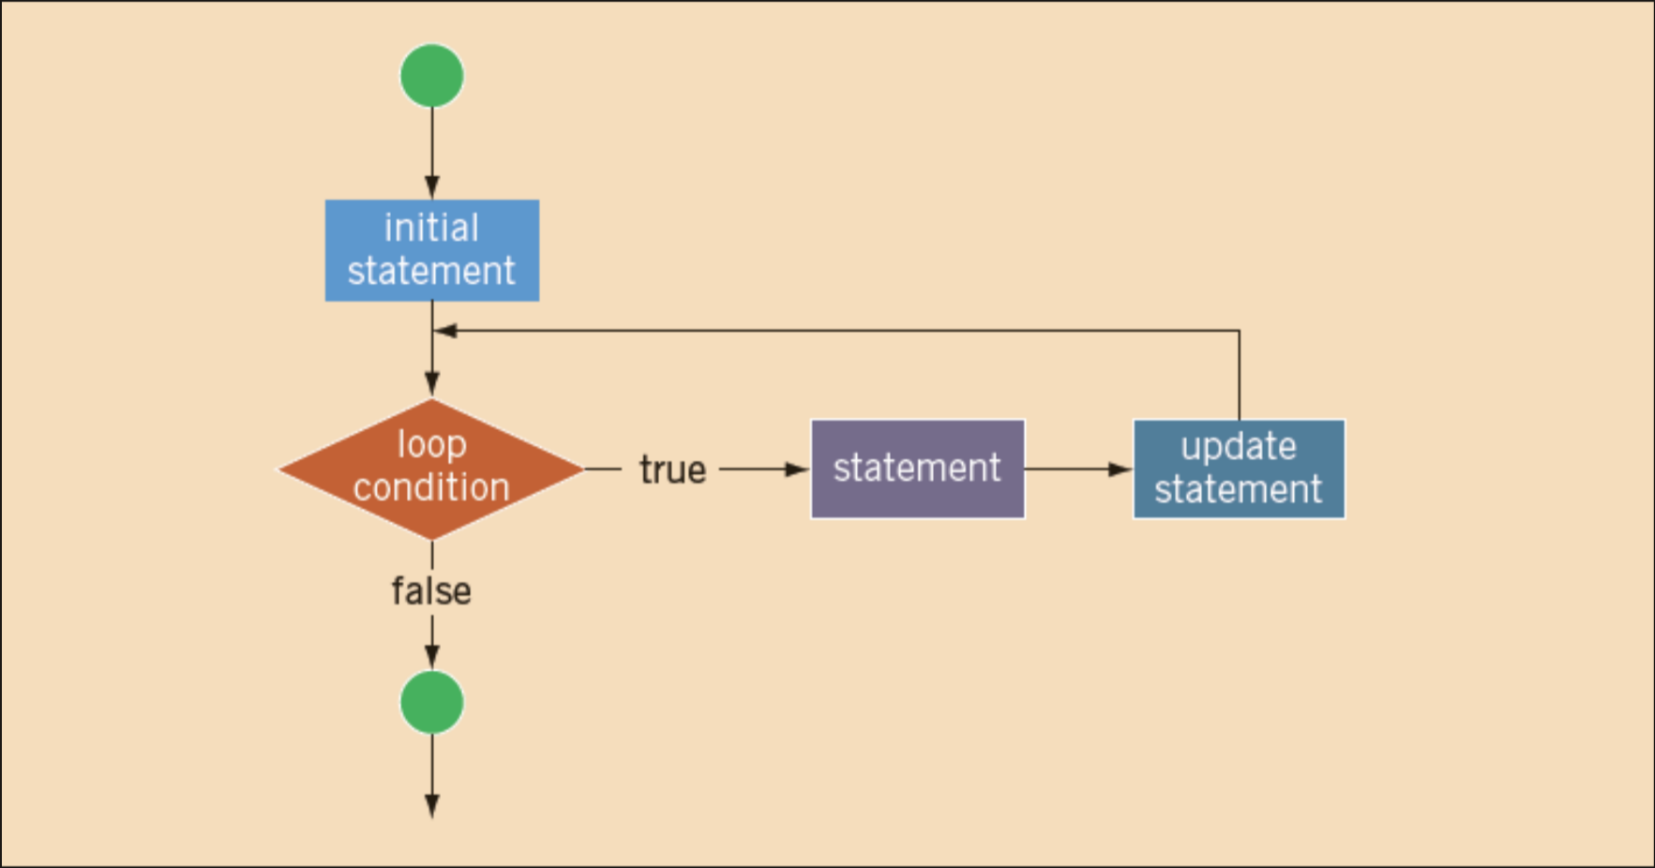
\includegraphics[width=0.9\textwidth]{for-exec-flow.png}
\end{center}

The \texttt{for} loop executes as follows:
\begin{enumerate}
  \item The \texttt{initial statement} executes.
  \item The \texttt{loop condition} is evaluated. If the \texttt{loop condition} evaluates
to \texttt{true}:
  \begin{itemize}
    \item Execute the \texttt{for} loop statement.
    \item Execute the \texttt{update statement}.
  \end{itemize}
\item Repeat \textit{Step 2} until the \texttt{loop condition} evaluates to 
    \texttt{false}.
\end{enumerate}

The \texttt{initial statement} usually initializes a variable (called the
\textbf{\texttt{for} loop control}, or \textbf{\texttt{for} indexed variable}).

\vspace{8pt}
Caveats:
\begin{itemize}
  \item If the \texttt{loop condition} is initially \texttt{false}, the loop body does not execute.
  \item The \texttt{for} loop body executes indefinitely if the \texttt{loop condition}
is always \texttt{true}.
  \item You can omit all three statements; however, the \texttt{for} statement
    must contain two semicolons \textit{(Listing 10)}.
\end{itemize}

\begin{lstlisting}[language=C++, caption={\texttt{for} Loop Gotcha}]
for (;;)
  cout << "Hello" << endl;
\end{lstlisting}

\section{\texttt{do..while} Looping (Repetition) Structure}

\begin{lstlisting}[language=C++, caption={\texttt{do..while} Loop Syntax}]
do
  statement
while(expression);
\end{lstlisting}
\textit{Statement can be a simple or compound statement.}

\vspace{8pt}
Execution Flow:
\begin{center}
    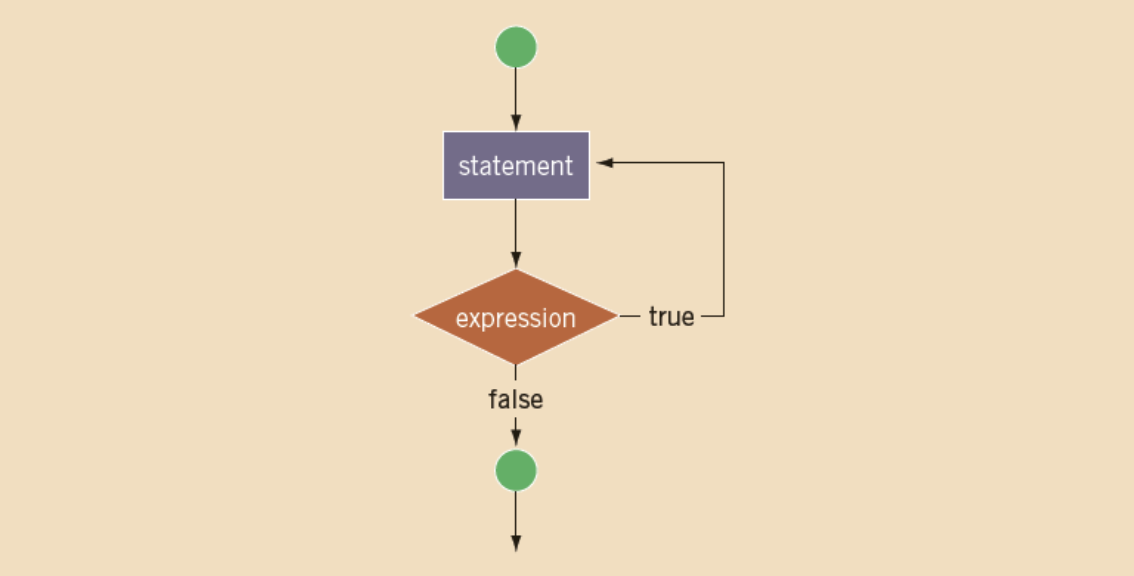
\includegraphics[width=0.9\textwidth]{do-while-exec-flow.png}
\end{center}

The \texttt{statement} executes first, then the \texttt{expression} is
evaluated.
\begin{itemize}
  \item As long as the \texttt{expression} evaluates to \texttt{true}, the loop
    continues.
\end{itemize}
In a \texttt{while} and \texttt{for} loop, the \texttt{loop condition} is
evaluated \textit{before} executing the body of the loop.
\begin{itemize}
  \item \texttt{while} and \texttt{for} loops are called \textbf{Pretest Loops}.
  \item \texttt{do...while} loops are called \textbf{Posttest Loops}.
\end{itemize}

\subsection{Choosing the Correct Looping Structure}
\begin{itemize}
  \item If you know the number of repetitions needed $\rightarrow$ \texttt{for} loop.
  \item If you do not know and it \textbf{could be 0} $\rightarrow$ \texttt{while} loop.
  \item If you do not know and it is \textbf{at least 1} $\rightarrow$ \texttt{do...while} loop.
\end{itemize}

\section{\texttt{break} and \texttt{continue} Statements}

\vspace{8pt}
The \texttt{break} statement is typically used for two purposes:
\begin{enumerate}
  \item To exit early from a loop.
  \item To skip the remainder of the \texttt{switch} structure.
\end{enumerate}

After the \texttt{break} statement executes, the program continues to execute
with the first statement after the structure.

\vspace{8pt}
The \texttt{continue} statement is used in all 3 loop structures:
\begin{enumerate}
  \item \texttt{while}
  \item \texttt{for}
  \item \texttt{do...while}
\end{enumerate}

When the \texttt{continue} statement is executed in a loop, it skips the
remaining statements in the loop and proceeds with the next iteration of the loop. 

\vspace{8pt}
Differences between loops:
\begin{itemize}
  \item \texttt{do..while} and \texttt{while} $\rightarrow$ \texttt{expression}
    is evaluated immediately after \allowbreak \texttt{continue} statement.
  \item \texttt{for} $\rightarrow$ \texttt{update statement} is executed after
    \texttt{continue} statement $\rightarrow$ \texttt{loop condition} executes.
\end{itemize}

\end{document}
